% Provenance (never printed): see sources/outline_sources.md (Year 3:
% facies analysis, depositional models, Walther's law, well logs). Brief:
% sources/book5/BRIEFS.md, ch. 17. Curves from figdata/bachelor-3/well_logs.py
% (unit tops from figdata/shared/region.py). Exercise and problem values in
% the Book 5 scratch calculator calc/ch17.py. The well वार्डन-2, its logs and
% the channel architecture of its sandstone are invented.
\chapter{संलक्षणी मॉडल}\label{ch:b3:facies-models}

एक किलोमीटर गहरे कुएँ का एक क्रोड: एक मीटर मोटी मोटे कण की रेत, जिसमें
तिर्यक संस्तरण हैं जो एक तीखे आधार पर टिके हैं, ऊपर की ओर महीन होकर मूलों के चिह्नों वाली गाद में
बदल जाती है, फिर दूसरे तीखे आधार पर रेत आ जाती है। भूवैज्ञानिक एक ऐसी नदी को पढ़ता है
जो अपने मैदान में घूमती रही, यद्यपि अब वहाँ कोई नदी नहीं बहती। यह व्याख्या
दो औज़ारों पर टिकी है: मॉडलों का एक समूह, जिनमें से प्रत्येक अनेक आधुनिक और
प्राचीन उदाहरणों का सारांश है, और एक नियम जो ऊर्ध्वाधर संस्तरों के अनुक्रम को
पड़ोसी परिवेशों के मानचित्र में बदल देता है।

\begin{recall}
अवसादी फ़ेसीज़, निक्षेपण-परिवेश, तल-आकृतियाँ, तिर्यक संस्तरण,
तीनों प्रकार के डेल्टा, गंदलाव-धाराएँ, गंदलाव-निक्षेप और क्रमित परतें
पुस्तक 3 (स्नातक वर्ष 1) में हैं, उसके उस अध्याय में जो कणकीय अवसादों और उनके
परिवेशों पर है; कार्बोनेट कारखाना, भित्तियाँ और कार्बोनेट प्लेटफ़ॉर्म उसके उस अध्याय में
हैं जो कार्बोनेट, सिलिसियस और वाष्पनिक अवसादों पर है; बोरहोल लॉग और
लॉग का सहसंबंध उसके उस अध्याय में है जो अनुप्रस्थ-काटों पर है। छिद्रता और
पारगम्यता स्कूली पुस्तकों में हैं। \omterm{def:b3:sequence-stratigraphy:parasequence}{पैरा-अनुक्रम}, प्लावन सतहें और
\omterm{def:b3:sequence-stratigraphy:tract}{तंत्र-पथ} अध्याय~\ref{ch:b3:sequence-stratigraphy} में हैं। गहरे पानी की तरंगें,
जिनकी गति गहराई के साथ घटती है, भौतिकी की पुस्तकों में हैं।
\end{recall}

\section{संलक्षणी, अनुक्रम और वाल्थर का नियम}\label{sec:b3:facies-models:walther}

अवसादी संलक्षणी का वर्णन उस पर आधारित है जो क्रोड या
कगार में दिखता है: कण-आकार, छँटाव, संरचनाएँ, जीवाश्म, रंग। एक अकेली संलक्षणी
शायद ही निदानात्मक होती है: तिर्यक-संस्तरित रेत नदियों में, पुलिनों पर, ज्वारीय
वाहिकाओं में और मरुस्थलों में बनती है। परिवेश की पहचान इस बात से होती है कि
कोई संलक्षणी किन संलक्षणियों के साथ रहती है और संलक्षणियाँ एक-दूसरे के बाद किस क्रम में आती हैं।

\begin{definition}[संलक्षणी साहचर्य और संलक्षणी अनुक्रम]\label{def:b3:facies-models:association}
\emph{संलक्षणी साहचर्य}\index{संलक्षणी साहचर्य} संलक्षणियों का एक समूह है
जो एक साथ पाई जाती हैं और एक ही परिवेश में निक्षेपित हुई हैं, जैसे वाहिका की रेत,
तटबंध की गाद और मूलों वाली बाढ़ के मैदान की पंक। एक \emph{संलक्षणी
अनुक्रम}\index{संलक्षणी अनुक्रम} संलक्षणियों का एक ऊर्ध्वाधर क्रम है, जिसमें कोई गुण
ऊपर की ओर क्रमशः बदलता है; एक \emph{ऊपर की ओर महीन होता
अनुक्रम}\index{ऊपर की ओर महीन होता अनुक्रम} में कण-आकार ऊपर की ओर घटता है,
और \emph{ऊपर की ओर स्थूल होता अनुक्रम}\index{ऊपर की ओर स्थूल होता अनुक्रम}
में यह बढ़ता है।
\end{definition}

\begin{definition}[संलक्षणी मॉडल]\label{def:b3:facies-models:model}
\emph{संलक्षणी मॉडल}\index{संलक्षणी मॉडल} एक सामान्य सारांश है
निक्षेपण-परिवेश का, जो अनेक आधुनिक और प्राचीन उदाहरणों से निकाला गया है:
वह जो संलक्षणियाँ उत्पन्न करता है, उनकी ज्यामिति, उनके पार्श्व संबंध,
और वे अनुक्रम जो वे बनाती हैं। यह एक मानक के रूप में काम आता है, जिससे नए उदाहरण की तुलना की जा सके,
आगे के प्रेक्षण का मार्गदर्शक, नई स्थितियों में पूर्वानुमान का साधन,
और परिवेश की व्याख्या का आधार।
\end{definition}

पार्श्व और ऊर्ध्वाधर को जोड़ने वाली कड़ी एक नियम है। पड़ोसी
परिवेश किसी भी क्षण साथ-साथ पड़े होते हैं: पुलिन \omterm{def:b3:facies-models:shoreface}{तटमुख} के बगल में,
\omterm{def:b3:facies-models:shoreface}{तटमुख} अपतटीय पंक के बगल में। जब तटरेखा खिसकती है,
तो प्रत्येक परिवेश अपने पड़ोसी के ऊपर आ जाता है।

\begin{theorem}[वाल्थर का नियम]\label{thm:b3:facies-models:walther}
अनुरूप अनुक्रम में, जहाँ निक्षेपण में कोई महत्वपूर्ण विराम या
अपरदन सतह न हो, वे संलक्षणियाँ जो एक-दूसरे के ठीक ऊपर स्थित हैं,
उन परिवेशों में निक्षेपित हुई थीं जो उस समय साथ-साथ पड़े थे।
\end{theorem}

\begin{proof}
मान लीजिए परिवेशों की पट्टियाँ हैं, प्रत्येक तटरेखा के समांतर एक पट्टी, जो
बेसिन के आर-पार एक साथ खिसकती हैं, जबकि तल अवधसित होता है या समुद्र-तल
उठता है। किसी स्थिर स्थान पर पट्टियाँ एक-एक करके गुज़रती हैं, उसी क्रम में
जिस क्रम में वे साथ-साथ पड़ी हैं, और हर पट्टी अपना निक्षेप
अपनी पूर्ववर्ती पट्टी के निक्षेप के ऊपर छोड़ती है। यदि निक्षेपण निरंतर है, तो
निक्षेपों का ऊर्ध्वाधर क्रम इसीलिए पट्टियों का पार्श्व क्रम है।
विराम या अपरदन सतह तर्क को बाधित करती है: विराम के दौरान जो पट्टियाँ गुज़रीं
उन्होंने कुछ नहीं छोड़ा, या उनके निक्षेप हटा दिए गए, और असन्निकट परिवेशों की
संलक्षणियाँ आपस में संपर्क में आ जाती हैं।
\end{proof}

\begin{omfigure}
\begin{tikzpicture}[font=\scriptsize, x=1cm, y=1cm]
% environments side by side, with a shoreline that moves seaward
\fill[yellow!35!brown!25] (0,0) rectangle (3,0.5);
\fill[yellow!30] (3,0) rectangle (4.4,0.5);
\fill[yellow!50!orange!30] (4.4,0) rectangle (6.4,0.5);
\fill[black!20] (6.4,0) rectangle (9,0.5);
\draw (0,0) rectangle (9,0.5);
\foreach \x in {3,4.4,6.4} {\draw (\x,0) -- (\x,0.5);}
\node at (1.5,0.25) {तटीय मैदान};
\node at (3.7,0.25) {पुलिन};
\node at (5.4,0.25) {तटमुख};
\node at (7.7,0.25) {अपतटीय पंक};
\draw[->, thick] (3.2,0.9) -- (5.2,0.9) node[right] {पट्टियाँ सागर की ओर खिसकती हैं};
\node[anchor=south] at (4.5,1.2) {(क) साथ-साथ पड़े परिवेश};
% vertical succession at a place
\begin{scope}[xshift=11cm, yshift=-1.2cm]
\fill[black!20] (0,0) rectangle (0.9,0.8);
\fill[yellow!50!orange!30] (0,0.8) -- (0.9,0.8) -- (1.3,1.8) -- (0,1.8) -- cycle;
\fill[yellow!30] (0,1.8) rectangle (1.4,2.4);
\fill[yellow!35!brown!25] (0,2.4) rectangle (1.0,3.1);
\draw (0,0) -- (0.9,0) -- (0.9,0.8) -- (1.3,1.8) -- (1.4,1.8) -- (1.4,2.4) -- (1.0,2.4) -- (1.0,3.1) -- (0,3.1) -- cycle;
\node[anchor=west] at (1.6,0.4) {अपतटीय पंक};
\node[anchor=west] at (1.6,1.3) {तटमुख की रेत};
\node[anchor=west] at (1.6,2.1) {पुलिन};
\node[anchor=west] at (1.6,2.75) {तटीय मैदान};
\draw[->] (-0.3,0) -- (-0.3,3.1) node[above] {ऊपर};
\node[anchor=north, align=center] at (0.9,-0.1) {(ख) एक स्थान पर\\ अनुक्रम};
\end{scope}
\end{tikzpicture}

\par\smallskip{\small वॉल्थर का नियम। (क) परिवेश किसी प्रोफ़ाइल के साथ-साथ एक-दूसरे की बगल में
स्थित होते हैं; (ख) जब पट्टियाँ समुद्र की ओर खिसकती हैं, तो एक स्थान पर अपतटीय पंक
आता है, फिर \omterm{def:b3:facies-models:shoreface}{तटमुख} की रेत, पुलिन की रेत और तटीय मैदान के निक्षेप: एक
\omterm{def:b3:facies-models:association}{ऊपर की ओर स्थूल होता अनुक्रम}, पट्टियों के क्रम में (लॉग में चौड़ाई
अधिक मोटे कण का अर्थ है)।}\label{fig:b3:facies-models:walther}
\end{omfigure}

यह नियम दोनों दिशाओं में लागू होता है। समुद्र के रिग्रेशन में पट्टियाँ अपने समुद्र की ओर के क्रम में
ऊपर की ओर ढेर होती हैं, जबकि ट्रांसग्रेशन में उल्टे क्रम में; और
क्रोड में पढ़ा गया ऊर्ध्वाधर अनुक्रम उस समय के निकटवर्ती परिवेशों का मानचित्र देता है। यह
ठीक वहीं विफल होता है, जहाँ अध्याय~\ref{ch:b3:sequence-stratigraphy} अपनी मुख्य सतहें रखता है:
\omterm{def:b3:sequence-stratigraphy:sequence}{अनुक्रम सीमा} के पार, जहाँ उद्भासन और अपरदन नदी की रेत को
मग्नतट के पंक पर ला रखते हैं, और \omterm{def:b3:sequence-stratigraphy:parasequence}{प्लावन सतह} के पार, जहाँ अपतटीय पंक
सीधे तटीय मैदान पर पड़ा होता है।

\section{नदियाँ}\label{sec:b3:facies-models:rivers}

\begin{definition}[गुंफित और विसर्पी नदियाँ]\label{def:b3:facies-models:rivers}
\emph{गुंफित नदी}\index{गुंफित नदी} कई उथली वाहिकाओं में बहती है, जो बार के चारों ओर बँटकर फिर मिल जाती हैं,
एक तीव्र ढाल वाले मैदान पर, जहाँ मोटे भार की प्रचुरता और
परिवर्ती विसर्जन होता है। \emph{विसर्पी नदी}\index{विसर्पी नदी}
एक ही घुमावदार वाहिका में बहती है, जो अपेक्षाकृत मंद ढाल वाले मैदान पर होती है,
अधिक महीन अवसाद ढोती है; यह हर मोड़ के बाहरी किनारे को काटकर
और भीतरी किनारे पर निक्षेप करके आगे बढ़ती है। भीतरी किनारे का निक्षेप एक \emph{बिंदु
पुलिन}\index{बिंदु-पुलिन}। \emph{अवल्शन}\index{अवल्शन} बाढ़ के मैदान के पार एक नए मार्ग के लिए वाहिका का त्याग है,
जो प्रायः तब होता है जब एक बाढ़
तटबंध को तोड़ देती है।
\end{definition}

\omterm{def:b3:facies-models:rivers}{बिंदु-पुलिन} पार्श्व में बढ़ता है, जब मोड़ खिसकता है, इसलिए किसी भी स्थान पर वह
वाहिका का अनुप्रस्थ काट नीचे से ऊपर तक दर्ज करता है: सबसे मोटे कंकड़ों का अवशेष-जमाव अपरदित आधार पर,
गहरी वाहिका के टिब्बों से आई तिर्यक संस्तरित रेत,
पुलिन के उथले शीर्ष से लहरिकाओं वाली महीन रेत, और फिर
जड़ों और मिट्टी के साथ बाढ़ के मैदान की गाद और पंक। वॉल्थर के नियम से यह
\omterm{def:b3:facies-models:association}{ऊपर की ओर महीन होता अनुक्रम}, जो कुछ मीटर मोटा है, मोटाई में
वाहिका की गहराई के बराबर होता है। \omterm{def:b3:facies-models:rivers}{गुंफित नदी} तिर्यक संस्तरित रेत की ढेरदार परतें छोड़ती है
और बजरी की, कम पंक के साथ, जिनका कण-आकार ऊपर की ओर लगभग नहीं बदलता; उसका महीन अंश
बह जाता है। \omterm{def:b3:facies-models:rivers}{अवल्शन} वाहिका-पट्टी को मैदान के पार इस प्रकार स्थानांतरित करता है,
कि वाहिका-निकाय बाढ़ के मैदान के पंकों के बीच यादृच्छिक रूप से ढेर हों, जिन्हें तीखे
अपरदनात्मक आधार अलग करते हैं।

\begin{omfigure}
\begin{tikzpicture}[font=\scriptsize, x=1cm, y=1cm]
% (क) braided plan
\begin{scope}
\fill[yellow!35!brown!20] (0,0) rectangle (4.6,2.4);
\draw[omDef!60, line width=1.6pt] (0,1.2) .. controls (0.8,1.6) and (1.4,0.6) .. (2.3,1.0) .. controls (3.0,1.3) and (3.6,0.7) .. (4.6,1.0);
\draw[omDef!60, line width=1.6pt] (0,1.2) .. controls (0.8,0.8) and (1.6,1.9) .. (2.4,1.6) .. controls (3.2,1.3) and (3.8,1.9) .. (4.6,1.6);
\draw[omDef!60, line width=1.2pt] (1.2,1.25) .. controls (1.8,1.5) and (2.6,1.2) .. (3.3,1.35);
\fill[yellow!45] (1.5,1.15) ellipse (0.35 and 0.12);
\fill[yellow!45] (3.0,1.25) ellipse (0.4 and 0.12);
\node[anchor=south] at (2.3,2.45) {(क) गुंफित};
\end{scope}
% (ख) meandering plan
\begin{scope}[xshift=5.4cm]
\fill[green!30!black!12] (0,0) rectangle (4.6,2.4);
\draw[omDef!60, line width=2pt] (0,1.2) .. controls (0.6,2.2) and (1.4,2.2) .. (1.6,1.2) .. controls (1.8,0.2) and (2.8,0.2) .. (3.0,1.2) .. controls (3.2,2.2) and (4.0,2.2) .. (4.6,1.2);
\fill[yellow!45] (0.8,1.45) ellipse (0.3 and 0.2);
\fill[yellow!45] (2.3,0.95) ellipse (0.3 and 0.2);
\fill[yellow!45] (3.8,1.45) ellipse (0.3 and 0.2);
\node at (2.3,0.95) {बिपु};
\draw[omDef!40, line width=1pt, densely dashed] (0.4,0.2) .. controls (1.0,0.7) and (1.6,0.4) .. (2.0,0.1);
\node[anchor=west, font=\tiny] at (2.6,2.15) {बाढ़ का मैदान};
\node[anchor=south] at (2.3,2.45) {(ख) विसर्पी};
\end{scope}
% logs
\begin{scope}[xshift=10.8cm]
\fill[yellow!45] (0,0) -- (1.2,0) -- (1.2,2.0) -- (0,2.0) -- cycle;
\draw (0,0) -- (1.2,0) -- (1.15,0.6) -- (1.2,0.65) -- (1.1,1.3) -- (1.2,1.35) -- (1.15,2.0) -- (0,2.0) -- cycle;
\node[anchor=north] at (0.6,-0.05) {गुंफित};
\end{scope}
\begin{scope}[xshift=12.6cm]
\fill[yellow!45] (0,0) -- (1.2,0) -- (1.1,0.9) -- (0.45,1.6) -- (0,1.6) -- cycle;
\fill[green!30!black!15] (0,1.6) rectangle (0.3,2.2);
\draw (0,0) -- (1.2,0) -- (1.1,0.9) -- (0.45,1.6) -- (0.3,1.6) -- (0.3,2.2) -- (0,2.2) -- cycle;
\draw[decorate, decoration={snake, amplitude=0.4mm, segment length=1.5mm}] (0,0) -- (1.2,0);
\node[anchor=north] at (0.6,-0.05) {बिंदु-पुलिन};
\node[anchor=west, font=\tiny] at (0.35,1.9) {जड़ें};
\end{scope}
\end{tikzpicture}

\par\smallskip{\small (क) \omterm{def:b3:facies-models:rivers}{गुंफित नदी}: बालू और बजरी के बारों के चारों ओर
कई वाहिकाएँ। (ख) \omterm{def:b3:facies-models:rivers}{विसर्पी नदी}: एक घुमावदार वाहिका, \omterm{def:b3:facies-models:rivers}{बिंदु-पुलिन} (बिपु)
भीतरी किनारों पर, \omterm{def:b3:facies-models:rivers}{अवल्शन} से छोड़ा गया एक त्यक्त मार्ग (बिंदीदार)। दाईं ओर:
अवसादों के कण-आकार के लॉग (चौड़ाई अधिक मोटे कण का अर्थ है): ढेरदार बालू-परतें,
ऊपर की ओर लगभग अपरिवर्तित, \omterm{def:b3:facies-models:rivers}{गुंफित नदी} के लिए; और तीखे
आधार वाला, \omterm{def:b3:facies-models:association}{ऊपर की ओर महीन होता अनुक्रम}, जिसे जड़ों वाले बाढ़-मैदान के पंक ने ढका है,
\omterm{def:b3:facies-models:rivers}{बिंदु-पुलिन} के लिए।}\label{fig:b3:facies-models:rivers}
\end{omfigure}

\section{तटरेखाएँ, डेल्टा और मग्नतट}\label{sec:b3:facies-models:shelves}

पुस्तक 3 (स्नातक वर्ष 1) के वे डेल्टा, जिन पर नदियों, तरंगों या ज्वारों का प्रभुत्व था, सभी
एक ही तंत्र से आगे बढ़ते हैं: मुहाना अपना भार वहीं जमा करता है, जहाँ धारा
मंद पड़ती है, और डेल्टा-अग्र अपने ही प्रोडेल्टा पंकों के ऊपर आगे बढ़ता है।
वॉल्थर के नियम से, आगे बढ़ता डेल्टा-अग्र या \omterm{def:b3:facies-models:shoreface}{तटमुख}
\omterm{def:b3:facies-models:association}{ऊपर की ओर स्थूल होता अनुक्रम} छोड़ता है: अपतटीय पंक, परस्पर-स्तरित पंक और तूफ़ान की रेत,
\omterm{def:b3:facies-models:shoreface}{तटमुख} की रेत, पुलिन। पिछले अध्याय का हर \omterm{def:b3:sequence-stratigraphy:parasequence}{पैरा-अनुक्रम} ऐसा ही एक
अनुक्रम है।

\begin{definition}[तटमुख और तरंग-आधार]\label{def:b3:facies-models:shoreface}
\emph{तटमुख}\index{तटमुख} वह ढालू क्षेत्र है, जो पुलिन के समुद्र की ओर स्थित है,
जहाँ तरंगें समुद्र-तल को लगातार पुनः संसाधित करती रहती हैं। इसका आधार
\emph{सामान्य-मौसम तरंग-आधार}\index{सामान्य-मौसम तरंग-आधार} है, वह गहराई जिसके नीचे
सामान्य तरंगें तल के अवसाद को अब नहीं हिलातीं। \emph{तूफ़ान
तरंग-आधार}\index{तूफ़ान तरंग-आधार} वह गहरी सीमा है जहाँ तूफ़ान की तरंगें पहुँचती हैं;
इन दोनों के बीच शांत मौसम में पंक जमता है, और वह रेत की परतों में पुनः संसाधित
होता है तूफ़ानों के दौरान। तूफ़ान तरंग-आधार के नीचे तल तरंगों से अविक्षुब्ध रहता है।
\end{definition}

\begin{omfigure}
\begin{tikzpicture}[font=\scriptsize, x=1cm, y=1.6cm]
\fill[omSea!60] (0,2.2) -- (13,2.2) -- (13,0.2) -- (5.5,0.9) -- (2.0,1.9) -- (0.6,2.2) -- cycle;
\fill[yellow!40] (0,2.4) -- (0.6,2.2) -- (2.0,1.9) -- (5.5,0.9) -- (5.5,0.0) -- (0,0.0) -- cycle;
\fill[black!18] (5.5,0.9) -- (13,0.2) -- (13,0) -- (5.5,0) -- cycle;
\draw[thick] (0,2.4) -- (0.6,2.2) -- (2.0,1.9) -- (5.5,0.9) -- (13,0.2);
\draw[omDef] (0,2.2) -- (13,2.2);
\draw[omDef, densely dashed] (1.6,1.97) -- (13,1.97);
\draw[omDef, densely dashed] (5.5,0.9) -- (13,0.9);
\node[omDef, anchor=north west] at (9.3,1.95) {फ़ेयर-वेदर तरंग-आधार};
\node[omDef, anchor=north west] at (9.3,0.88) {तूफ़ान तरंग-आधार};
\node[anchor=south] at (0.5,2.42) {पुलिन};
\node at (1.8,1.35) {तटमुख};
\node at (4.3,0.45) {अपतट संक्रमण};
\node at (9.0,0.15) {अपतट पंक};
\node[align=center] at (7.4,1.45) {तूफ़ान रेत-संस्तर,\\ टीलेदार तिर्यक स्तरण};
\end{tikzpicture}

\par\smallskip{\small तरंग-प्रधान तटरेखा परिच्छेद (योजनाबद्ध, ऊर्ध्वाधर
पैमाना बहुत बढ़ाया गया)। \omterm{def:b3:facies-models:shoreface}{सामान्य-मौसम तरंग-आधार} के ऊपर \omterm{def:b3:facies-models:shoreface}{तटमुख} की रेत
हर दिन पुनः संसाधित होती है; दोनों तरंग-आधारों के बीच पंक
तूफ़ान-जनित रेत-संस्तरों के साथ एकांतर क्रम में आता है; \omterm{def:b3:facies-models:shoreface}{तूफ़ान तरंग-आधार} के नीचे पंक
संचित होता है।}\label{fig:b3:facies-models:shoreface}
\end{omfigure}

गहरे जल में तरंग की कक्षीय गति $e^{-2\pi z/\lambda}$ के अनुसार घटती है,
गहराई $z$ पर, तरंगदैर्घ्य $\lambda$ के लिए: आधे तरंगदैर्घ्य पर वह
\qty{4}{\percent} अपने सतह-आयाम का बनाए रखती है, और यही तरंग-आधार का पैमाना तय करता है।
कैरिबियन, मेक्सिको की खाड़ी और पश्चिमी अटलांटिक के दो मिलियन से अधिक तरंग-स्पेक्ट्रम के बॉय-अभिलेख
प्रमुख तरंगदैर्घ्य
संरक्षित समुद्रों में लगभग \qty{75}{m} और खुले किनारे पर लगभग \qty{110}{m} बताते हैं,
और दिखाते हैं कि सप्ताहों से वर्षों के औसत पर तरंगदैर्घ्य
सामान्य-मौसम वर्ग और तूफ़ान वर्ग में नहीं बँटते: किसी तरंग द्वारा तल को हिलाने की
संभावना उथले होते पानी के साथ लगातार बढ़ती है। दोनों तरंग-आधार अब भी उपयोगी शब्द बने रहते हैं
परिच्छेद के क्षेत्रों के लिए, तीखी गहराइयों के लिए नहीं।
% ledger: losspeters10:wavebase

\begin{definition}[टीलेदार तिर्यक स्तरण]\label{def:b3:facies-models:hcs}
\emph{टीलेदार तिर्यक स्तरण}\index{टीलेदार तिर्यक स्तरण} महीन रेत का एक स्तरीकरण है, जो
मंद रूप से वक्र पट्टिकाओं में होता है, जो अवतल-ऊपर (गर्त) और उत्तल-ऊपर (टीले)
आकृतियाँ बनाती हैं, जो एक-दूसरे को निम्न कोणों पर काटती हैं और
पार्श्वतः मोटी और पतली होती हैं; इनकी तरंगदैर्घ्य एक मीटर से कई मीटर तक होती है। यह
तूफ़ान तरंगों के दोलनी और संयुक्त प्रवाहों से बनता है, जो
सामान्य-मौसम और \omterm{def:b3:facies-models:shoreface}{तूफ़ान तरंग-आधार} के बीच होता है।
\end{definition}

\begin{inthefield}[सिल्यूरियन मग्नतट पर तूफ़ान-संस्तर]
\begin{minipage}[t]{0.42\linewidth}\vspace{0pt}
नोवा स्कॉटिया की एरिसाइग संरचना में महीन बलुआ पत्थर की परतें
अधिक गहरे रंग के पंकाश्म को अलग करती हैं। ऐसे संस्तरों का अध्ययन करने वाले भूवैज्ञानिक निम्न, वक्र,
परस्पर काटती हुई \omterm{def:b3:facies-models:hcs}{टीलेदार तिर्यक स्तरण} की पट्टिकाएँ पहचानते हैं: हर संस्तर उस तूफ़ान का अभिलेख है
जिसने रोज़मर्रा की तरंगों की पहुँच से नीचे मग्नतट को हिलाया, और उसके आसपास का पंक
तूफ़ानों के बीच की लंबी शांति का।
\end{minipage}\hfill
\begin{minipage}[t]{0.54\linewidth}\vspace{0pt}
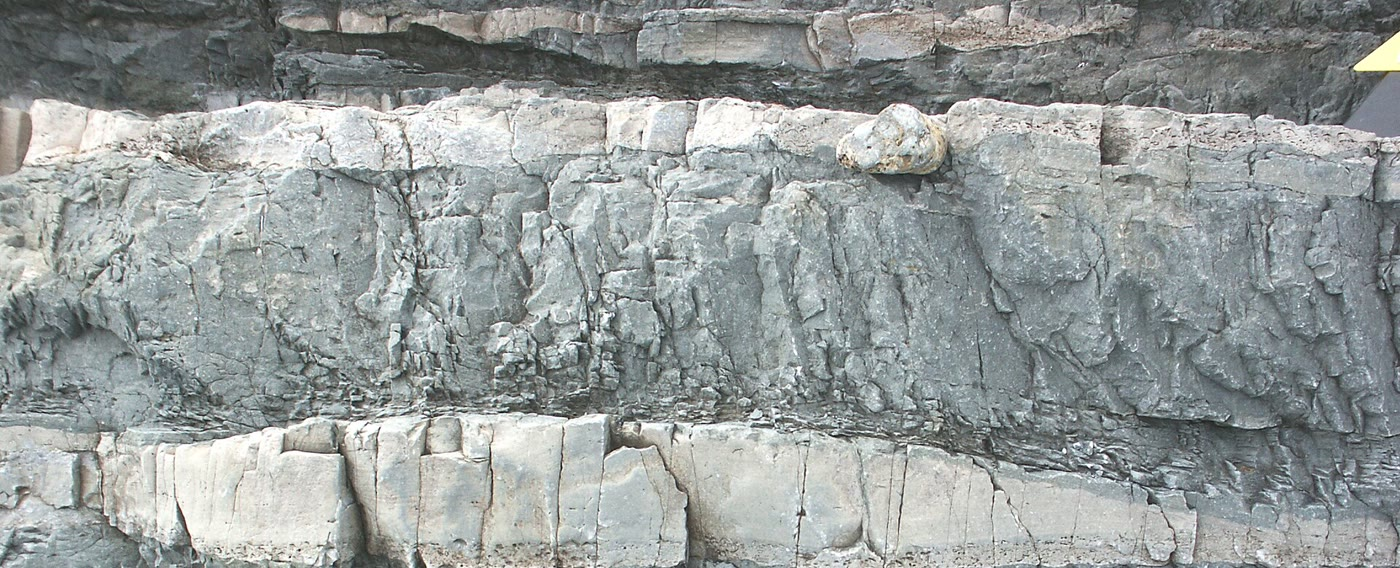
\includegraphics[width=\linewidth]{images/book5/b3-hummocky-cross-stratification.jpg}

{\scriptsize एरिसाइग संरचना में \omterm{def:b3:facies-models:hcs}{टीलेदार तिर्यक स्तरण}
(सिल्यूरियन), एरिसाइग के पास, नोवा स्कॉटिया। फ़ोटो: Michael C. Rygel, CC BY-SA 3.0
(काटा गया)।}
\end{minipage}
\end{inthefield}
% ledger: photo:b3-hcs

जहाँ ज्वार प्रबल होते हैं, वहाँ संलक्षणी बदल जाती है: बाढ़ और भाटा की धाराएँ
तिर्यक संस्तर बनाती हैं जो विपरीत दिशाओं में झुकते हैं, और हर शिथिल जल पर पंक-आवरण जमते हैं
शिथिल जल पर। आवरणों के बीच के समूहों की मोटाई
ज्वार के वृहत् और लघु चक्र के साथ घटती-बढ़ती है। ज्वारीय वाहिकाएँ, ज्वारीय मैदान और रेत-कटक
अपने-अपने मॉडल रखते हैं, जो इसी ढंग से बनते हैं।

\section{गहरा जल}\label{sec:b3:facies-models:deep}

मंद पड़ती गंदलाव-धारा अपना भार अवसादन के क्रम में निक्षेपित करती है:
सबसे मोटे कण पहले, सबसे महीन कण अंत में। एक पूर्ण गंदलाव-निक्षेप संस्तर इस क्रम को
पाँच भागों में दिखाता है।

\begin{definition}[बोमा अनुक्रम]\label{def:b3:facies-models:bouma}
\emph{बोमा अनुक्रम}\index{बोमा अनुक्रम} गंदलाव-निक्षेप संस्तर में भागों का आदर्श
क्रम है, आधार से शीर्ष तक: Ta, अपरदित आधार पर फ़्लूट और औज़ार-चिह्नों वाली सघन या क्रमित रेत;
Tb, समानांतर-पट्टित रेत; Tc,
लहरिका-तिर्यक पट्टित और कुंचित महीन रेत; Td, समानांतर-पट्टित गाद;
Te, पंक, जो अंशतः गंदलाव-धारा से और अंशतः
प्रवाहों के बीच धीमे अवसादन से आता है।
\end{definition}

कुछ ही संस्तर पाँचों भाग दिखाते हैं: स्रोत के निकट धारा तीव्र होती है और मोटे Ta भाग छोड़ जाती है,
जिनके ऊपरी भाग अगले प्रवाह से अपरदित हो जाते हैं; उससे दूर केवल
महीन भाग, Tc से Te तक, पहुँचते हैं। इस प्रकार अनुक्रम एक प्रवाह के
क्षीण होने का अभिलेख रखता है, और पंखे के साथ संस्तरों का बदलाव प्रवाहों के
दूरी के साथ क्षीण होने का।

\begin{definition}[जलमग्न पंखा]\label{def:b3:facies-models:fan}
\emph{जलमग्न पंखा}\index{जलमग्न पंखा} महाद्वीपीय ढाल के आधार पर अवसाद का एक शंकु है,
जिसे एक कैनियन पोषित करता है: तटबंधों के बीच मुख्य वाहिका वाला ऊपरी पंखा,
रेत-लोबों पर समाप्त होती वितरिका-वाहिकाओं वाला मध्य पंखा,
और पतले गंदलाव-निक्षेपों वाला निचला पंखा, जो बेसिन-तल के पंक में बदल जाता है।
\end{definition}

किनारे के साथ, महासागरीय परिसंचरण से चालित गहरी धाराएँ ढाल के
महीन अवसाद को कंटूराइट, टीलों और ड्रिफ़्ट में बदल देती हैं, जो जैव-विक्षुब्ध गाद और
पंक से बने होते हैं और समोच्च-रेखाओं के साथ बढ़ते हैं, ढाल की दिशा में
नीचे की ओर नहीं।

\begin{omfigure}
\begin{tikzpicture}[font=\scriptsize, x=1cm, y=1cm]
% (क) Bouma log
\begin{scope}
\fill[yellow!45] (0,0) -- (1.6,0) -- (1.6,1.2) -- (0,1.2) -- cycle;
\fill[yellow!35] (0,1.2) rectangle (1.3,1.8);
\fill[yellow!25] (0,1.8) rectangle (1.0,2.4);
\fill[black!12] (0,2.4) rectangle (0.7,2.8);
\fill[black!25] (0,2.8) rectangle (0.4,3.3);
\draw (0,0) -- (1.6,0) -- (1.6,1.2) -- (1.3,1.2) -- (1.3,1.8) -- (1.0,1.8) -- (1.0,2.4) -- (0.7,2.4) -- (0.7,2.8) -- (0.4,2.8) -- (0.4,3.3) -- (0,3.3) -- cycle;
\draw[decorate, decoration={snake, amplitude=0.5mm, segment length=2mm}] (0,0) -- (1.6,0);
\foreach \y in {1.35,1.5,1.65} {\draw[black!60] (0.05,\y) -- (1.25,\y);}
\foreach \x in {0.15,0.45,0.75} {\draw[black!60] (\x,1.95) .. controls (\x+0.08,2.1) .. (\x+0.2,1.95);}
\foreach \y in {2.5,2.6,2.7} {\draw[black!60] (0.05,\y) -- (0.65,\y);}
\foreach \y/\t in {0.6/Ta, 1.5/Tb, 2.1/Tc, 2.6/Td, 3.05/Te} {\node[anchor=west] at (1.9,\y) {\t};}
\node[anchor=west, align=left, font=\tiny] at (2.4,0.6) {सघन या क्रमित रेत,\\ अपरदित आधार};
\node[anchor=west, font=\tiny] at (2.4,1.5) {समानांतर पट्टिकाएँ};
\node[anchor=west, font=\tiny] at (2.4,2.1) {लहरिकाएँ, कुंचित पट्टिकाएँ};
\node[anchor=west, font=\tiny] at (2.4,2.6) {पट्टित गाद};
\node[anchor=west, font=\tiny] at (2.4,3.05) {पंक};
\node[anchor=north] at (1.6,-0.15) {(क) एक गंदलाव-निक्षेप संस्तर};
\end{scope}
% (ख) fan plan
\begin{scope}[xshift=8.2cm, yshift=0.2cm]
\fill[black!8] (-1.0,-0.2) rectangle (5.6,3.1);
\fill[yellow!20] (0.3,2.9) .. controls (1.6,2.6) and (4.9,2.0) .. (5.2,0.9) .. controls (4.6,-0.1) and (1.2,0.1) .. (0.3,1.6) -- cycle;
\fill[yellow!45] (1.9,1.9) ellipse (0.55 and 0.3);
\fill[yellow!45] (2.6,1.0) ellipse (0.55 and 0.3);
\fill[yellow!45] (3.4,1.75) ellipse (0.5 and 0.28);
\draw[omDef, line width=1.4pt] (-0.9,3.0) .. controls (-0.3,2.8) and (0.4,2.6) .. (1.0,2.2);
\draw[omDef, line width=0.8pt] (1.0,2.2) -- (1.6,1.95);
\draw[omDef, line width=0.8pt] (1.0,2.2) -- (2.3,1.15);
\draw[omDef, line width=0.8pt] (1.0,2.2) .. controls (2.0,2.4) .. (3.1,1.85);
\node[anchor=south west] at (-0.95,3.0) {कैनियन};
\node[anchor=east] at (0.55,2.0) {तटबंध};
\node[align=center, font=\tiny] at (2.6,1.0) {लोब};
\node at (4.4,0.7) {निचला पंखा};
\node[black!60] at (4.9,2.85) {बेसिन-तल};
\node[anchor=north] at (2.3,-0.25) {(ख) योजना में एक जलमग्न पंखा};
\end{scope}
\end{tikzpicture}

\par\smallskip{\small (क) एक पूर्ण गंदलाव-निक्षेप संस्तर का \omterm{def:b3:facies-models:bouma}{बोमा अनुक्रम},
कण-आकार लॉग के रूप में खींचा गया (चौड़ाई अधिक स्थूल का अर्थ देती है), इसके पाँच खंडों सहित। (ख)
योजना में एक \omterm{def:b3:facies-models:fan}{जलमग्न पंखा}: एक कैनियन तटबंधों के बीच की एक वाहिका की आपूर्ति करता है, जो
बँटकर रेत के लोबों पर समाप्त होने वाली वितरिका वाहिकाओं में विभाजित होती है;
पतले गंदलाव-निक्षेप निचले पंखे पर फैले होते हैं।}\label{fig:b3:facies-models:deep}
\end{omfigure}

\section{कार्बोनेट प्लेटफ़ॉर्म}\label{sec:b3:facies-models:carbonates}

कार्बोनेट अवसाद उथले, गर्म और स्वच्छ पानी में जीवों द्वारा,
जहाँ वह पड़ा होता है वहीं बनता है, और इसकी संलक्षणियाँ उस प्लेटफ़ॉर्म की रूपरेखा का अनुसरण करती हैं जिसे
कार्बोनेट कारखाना अपने लिए बनाता है।

\begin{definition}[कार्बोनेट रैंप और कगारयुक्त मग्नतट]\label{def:b3:facies-models:ramp}
\emph{कार्बोनेट रैंप}\index{कार्बोनेट रैंप} एक ऐसा प्लेटफ़ॉर्म है जिसका तल
तटरेखा से बेसिन की ओर बिना किसी विराम के, धीरे और समान रूप से ढलता है:
इसकी संलक्षणी पट्टियाँ, ज्वारीय मैदानों और पुलिन-अवरोधक रेत से लेकर उथले कणों तक,
जैव-खंडित रेत और अपतटीय चूना-कीचड़ तक, चौड़ी हैं और धीरे-धीरे एक-दूसरे में बदल जाती हैं,
गहराई के साथ घटती तरंग-ऊर्जा द्वारा छँटी हुई। एक \emph{कगारयुक्त
मग्नतट}\index{कगारयुक्त मग्नतट} एक सपाट-शीर्ष प्लेटफ़ॉर्म है, जिसके किनारे पर ढाल में एक स्पष्ट विराम होता है,
जहाँ भित्तियाँ और रेत के उथले टीले एक ऐसा कगार बनाते हैं जो
उसके पीछे एक लैगून को आश्रय देता है; कगार के परे का तीव्र ढाल ब्लॉकों और कणों को
बेसिन में गिराता है।
\end{definition}

\begin{omfigure}
\begin{tikzpicture}[font=\scriptsize, x=1cm, y=1cm]
\begin{scope}
\fill[omSea!60] (0,1.6) -- (6.4,1.6) -- (6.4,0.3) -- cycle;
\fill[black!10] (0,1.6) -- (6.4,0.3) -- (6.4,0) -- (0,0) -- cycle;
\draw[thick] (0,1.7) -- (0.3,1.6) -- (6.4,0.3);
\draw[omDef] (0,1.6) -- (6.4,1.6);
\node[anchor=south] at (0.6,1.65) {ज्वारीय मैदान};
\node[rotate=-12, font=\tiny] at (1.5,1.08) {उथले कण};
\node[rotate=-12, font=\tiny] at (3.4,0.66) {जैव-खंडित रेत};
\node[rotate=-12, font=\tiny] at (5.3,0.26) {चूना-कीचड़};
\node[anchor=north] at (3.2,-0.1) {(क) रैंप: समान ढाल, क्रमिक पट्टियाँ};
\end{scope}
\begin{scope}[xshift=7.2cm]
\fill[omSea!60] (0,1.6) -- (6.4,1.6) -- (6.4,0.2) -- (4.4,0.3) -- (3.6,1.55) -- (3.2,1.6) -- (0.3,1.6) -- cycle;
\fill[omSea!60] (0.3,1.6) -- (3.2,1.6) -- (3.0,1.35) -- (0.6,1.35) -- cycle;
\fill[black!10] (0,1.7) -- (0.3,1.6) -- (0.6,1.35) -- (3.0,1.35) -- (3.2,1.6) -- (3.6,1.55) -- (4.4,0.3) -- (6.4,0.2) -- (6.4,0) -- (0,0) -- cycle;
\draw[thick] (0,1.7) -- (0.3,1.6) -- (0.6,1.35) -- (3.0,1.35) -- (3.2,1.6) -- (3.6,1.55) -- (4.4,0.3) -- (6.4,0.2);
\fill[orange!50] (3.05,1.4) -- (3.2,1.6) -- (3.55,1.56) -- (3.6,1.4) -- cycle;
\draw[omDef] (0,1.6) -- (6.4,1.6);
\node at (1.8,1.12) {लैगून};
\node[anchor=south] at (3.35,1.65) {भित्ति-कगार};
\node[anchor=west] at (4.2,0.95) {तीव्र ढाल};
\node at (5.5,0.6) {बेसिन};
\node[anchor=north] at (3.2,-0.1) {(ख) कगारयुक्त मग्नतट: कगार, लैगून, ढाल};
\end{scope}
\end{tikzpicture}

\par\smallskip{\small कार्बोनेट प्लेटफ़ॉर्म की रूपरेखाएँ (योजनाबद्ध, ऊर्ध्वाधर पैमाना
बहुत बढ़ा-चढ़ाकर दिखाया गया)। (क) एक रैंप: समान ढाल के साथ तरंग-ऊर्जा द्वारा छाँटी गई
पट्टियाँ। (ख) एक \omterm{def:b3:facies-models:ramp}{कगारयुक्त मग्नतट}: ढाल-विराम पर एक भित्ति और उथले टीलों का कगार
चूना-कीचड़ के एक लैगून को आश्रय देता है; उसके परे का ढाल
कगार से गिरे ब्लॉकों और कणों को ग्रहण करता है।}\label{fig:b3:facies-models:platforms}
\end{omfigure}

समतल प्लेटफ़ॉर्म-शीर्ष पर सापेक्ष समुद्र-तल की एक छोटी वृद्धि ज्वारीय
मैदानों को जलमग्न कर देती है, और सबसे उथले पानी में सबसे तेज़ काम करने वाला कारखाना,
उस स्थान को थोड़े समय में फिर से समुद्र-तल तक भर देता है। इसका परिणाम पेरिटाइडल चक्रों का एक ऐसा ढेर है,
जिसकी मोटाई एक मीटर या कुछ मीटर होती है, और प्रत्येक एक ऊपर की ओर उथला होता \omterm{def:b3:sequence-stratigraphy:parasequence}{पैरा-अनुक्रम} है,
जो उपज्वारीय कीचड़ से लेकर सूखन-दरारों या सूक्ष्मजैविक चटाइयों वाले ज्वारीय मैदान तक जाता है,
और जिसके ऊपर अगली \omterm{def:b3:sequence-stratigraphy:parasequence}{प्लावन सतह} आती है।

\section{क्रोड और कुआँ-लॉग}\label{sec:b3:facies-models:logs}

अवसादी द्रोणियों के नीचे की अधिकांश चट्टानें बोरछिद्रों से ज्ञात होती हैं। इनमें से कुछ
के क्रोड निकाले गए हैं, और उनका वर्णन कगार की भाँति संस्तर-दर-संस्तर किया जाता है; लगभग सभी
का लॉग बनाया गया है।

\begin{definition}[वायरलाइन लॉग]\label{def:b3:facies-models:wireline}
\emph{वायरलाइन लॉग}\index{वायरलाइन लॉग} चट्टानों के किसी भौतिक गुणधर्म का गहराई के सापेक्ष एक सतत अभिलेख है,
जिसे बोरछिद्र में केबल पर नीचे उतारे गए एक प्रोब से मापा जाता है।
\emph{गामा-किरण लॉग}\index{गामा-किरण लॉग} चट्टान के प्राकृतिक गामा विकिरण को API इकाइयों में अभिलिखित करता है:
शेल में ऊँचा मान, जिसकी मिट्टियों में पोटैशियम, थोरियम और यूरेनियम होते हैं,
और स्वच्छ क्वार्ट्ज़ रेत तथा चूना-पत्थर में निम्न मान।
\emph{घनत्व-लॉग}\index{घनत्व-लॉग} सकल घनत्व अभिलिखित करता है, जो प्रोब पर स्थित एक स्रोत से उत्सर्जित
गामा-किरणों के प्रकीर्णन से निकाला जाता है।
\emph{ध्वनिक लॉग}\index{ध्वनिक लॉग} संपीडन तरंग के अंतराल पारगमन समय को,
प्रति फ़ुट माइक्रोसेकंड में, अभिलिखित करता है।
\emph{न्यूट्रॉन लॉग}\index{न्यूट्रॉन लॉग} न्यूट्रॉनों के हाइड्रोजन द्वारा मंदन को
और इस प्रकार छिद्रों और मिट्टियों में धारित जल को अभिलिखित करता है।
\end{definition}
% ledger: keys:gamma, keys:density-porosity, keys:sonic

API गामा-किरण इकाई एक अंशांकन गड्ढे में परिभाषित होती है: दो-सौवाँ भाग
नगण्य रेडियोधर्मिता वाले क्षेत्र और ऐसे क्षेत्र के बीच के अंतर का, जिसमें औसत शेल के
रेडियोसमस्थानिक लगभग दोगुने सांद्रण पर होते हैं। कोयला,
चूना-पत्थर और डोलोमाइट आमतौर पर शेल से कम रेडियोधर्मी होते हैं; क्वार्ट्ज़
बलुआ पत्थर निम्न है, पोटैशियम फ़ेल्सपार से समृद्ध आर्कोज़ ऊँचा; कोई भी चट्टान
भूजल द्वारा बहाकर लाए गए यूरेनियम से रेडियोधर्मी बनाई जा सकती है।
% ledger: keys:gamma

\begin{proposition}[घनत्व और पारगमन समय से छिद्रता]\label{prop:b3:facies-models:porosity}
छिद्रता $\phi$ वाली एक चट्टान, जिसके कण $\rho_{\mathrm{ma}}$ घनत्व के हैं और
जिसके रंध्र $\rho_f$ घनत्व वाले तरल से भरे हैं, उसका सकल घनत्व
$\rho_b = (1 - \phi)\rho_{\mathrm{ma}} + \phi\rho_f$ होता है, जिससे
\[
\phi = \frac{\rho_{\mathrm{ma}} - \rho_b}{\rho_{\mathrm{ma}} - \rho_f}.
\]
यदि एक संपीडन तरंग कणों और तरल को श्रेणी में पार करती है,
जिनकी लंबाइयाँ $1 - \phi$ और $\phi$ के समानुपाती हैं, उसका पारगमन समय
$\Delta t = (1 - \phi)\Delta t_{\mathrm{ma}} + \phi\Delta t_f$ होता है (समय-औसत
समीकरण), और $\phi = (\Delta t - \Delta
t_{\mathrm{ma}})/(\Delta t_f - \Delta t_{\mathrm{ma}})$।
\end{proposition}

\begin{proof}
एक इकाई आयतन की चट्टान में $1 - \phi$ आयतन कणों का और $\phi$ आयतन तरल का होता है;
उसका द्रव्यमान $(1 - \phi)\rho_{\mathrm{ma}} + \phi\rho_f$ है, इसलिए इसे
$\phi$ के लिए हल किया जाता है। तरंग के लिए, इकाई लंबाई का पथ $1 - \phi$ कणों को
और $\phi$ तरल को पार करता है, और समय जुड़ते हैं।
\end{proof}

कणों के घनत्व क्वार्ट्ज़ के लिए \qty{2.65}{g/cm^3} और चूना-पत्थर के लिए \qty{2.71}{g/cm^3} हैं;
रंध्र का जल ताज़ा होने पर \qty{1.0}{g/cm^3} और
खारे जल में \qty{1.1}{g/cm^3} तक। पारगमन समय 42 से
\qty{48}{\micro\second/ft} तक डोलोमाइट में, चूना-पत्थर में 48 से 53;
संपीड़ित बलुआ पत्थर के लिए 53, और खारे जल के लिए 189 है। घनत्व समीकरण
ज्ञात आव्यूह के लिए यथार्थ है; समय-औसत समीकरण एक अनुभवजन्य नियम है, जो
अंतराकणीय रंध्रों वाली संपीड़ित चट्टानों में सबसे अच्छा काम करता है। शेल दोनों को
विफल करता है: मृत्तिकाओं के अपने घनत्व होते हैं और वे बद्ध जल रखती हैं।
% ledger: keys:density-porosity, keys:sonic

\begin{definition}[शुद्ध-से-सकल अनुपात]\label{def:b3:facies-models:ntg}
किसी अंतराल का \emph{शुद्ध-से-सकल अनुपात}\index{शुद्ध-से-सकल अनुपात} उसकी जलाशय-गुणवत्ता वाली चट्टान की
मोटाई है, जो आमतौर पर \omterm{def:b3:facies-models:wireline}{गामा-किरण
लॉग} पर एक सीमा से नीचे चुनी गई रेत होती है, जिसे अंतराल की कुल मोटाई से भाग दिया जाता है।
\end{definition}

किसी रेत-निकाय के माध्यम से गामा-किरण वक्र का आकार एक संलक्षणी उपकरण है।
एक \emph{घंटी}, जो आधार पर साफ़ और ऊपर की ओर अधिक शेलयुक्त है, \omterm{def:b3:facies-models:association}{ऊपर की ओर महीन होता अनुक्रम} है,
जैसा \omterm{def:b3:facies-models:rivers}{बिंदु-पुलिन} या वाहिका-भराव में होता है; एक \emph{कीप}, जो आधार पर शेलयुक्त और
शीर्ष पर साफ़ है, \omterm{def:b3:facies-models:association}{ऊपर की ओर स्थूल होता अनुक्रम} है, जैसा प्रगामी \omterm{def:b3:facies-models:shoreface}{तटमुख} या
डेल्टा-अग्रभाग में होता है; एक \emph{बेलन}, जो पूरी लंबाई में साफ़ है और
तीखी सीमाएँ रखता है, एक ढेरित गुंफित-नदी रेत, एक वायु-निक्षेपित टिब्बा या एक
कार्बोनेट शोल है। ये आकार संकेत हैं, प्रमाण नहीं: इनकी पुष्टि के लिए एक क्रोड, या कम से कम
पड़ोसी लॉग, ज़रूरी हैं।

\begin{omfigure}
\begin{tikzpicture}
\begin{groupplot}[group style={group size=3 by 1, horizontal sep=0.2cm,
    y descriptions at=edge left},
  omrecord, y dir=reverse, ymin=700, ymax=1200, width=0.28\linewidth,
  height=0.62\linewidth, ytick={700,800,900,1000,1100,1200},
  tick label style={font=\scriptsize}, label style={font=\small},
  xlabel style={font=\small}]
\nextgroupplot[xlabel={GR (API)}, ylabel={गहराई (m)}, xmin=0, xmax=150,
  xtick={0,50,100,150}]
\addplot[black!60, densely dashed, forget plot] coordinates {(60,1046) (60,1166)};
% computed in figdata/bachelor-3/well_logs.py
\addplot[omDef, thin] table[x=gr, y=depth] {figdata/out/bachelor-3-well_logs-logs.dat};
\node[font=\scriptsize, anchor=west] at (axis cs:2,730) {चॉक};
\node[font=\scriptsize, anchor=west] at (axis cs:2,816) {शेल};
\node[font=\scriptsize, anchor=west] at (axis cs:28,956) {चूना-पत्थर};
\node[font=\scriptsize, anchor=west] at (axis cs:28,1030) {बलुआ पत्थर};
\node[font=\scriptsize, anchor=west] at (axis cs:2,1185) {शिस्ट};
\nextgroupplot[xlabel={$\rho_b$ (\unit{g/cm^3})}, xmin=1.9, xmax=2.9,
  xtick={2.0,2.4,2.8}, xticklabels={2.0,2.4,2.8}]
\addplot[red!70!black, thin] table[x=rhob, y=depth] {figdata/out/bachelor-3-well_logs-logs.dat};
\nextgroupplot[xlabel={$\Delta t$ (\unit{\micro\second/ft})}, xmin=40, xmax=140,
  x dir=reverse, xtick={40,80,120}]
\addplot[green!40!black, thin] table[x=dt, y=depth] {figdata/out/bachelor-3-well_logs-logs.dat};
\end{groupplot}
\begin{axis}[at={(group c3r1.south east)}, xshift=1.35cm, anchor=south west,
  omrecord, y dir=reverse, ymin=1040, ymax=1172, width=0.28\linewidth,
  height=0.62\linewidth, xmin=0, xmax=120, xtick={0,60,120},
  ytick={1040,1060,1080,1100,1120,1140,1160}, ylabel={गहराई (m)},
  xlabel={GR (API), बलुआ पत्थर}, tick label style={font=\scriptsize},
  label style={font=\small}]
\addplot[black!60, densely dashed, forget plot] coordinates {(60,1046) (60,1166)};
\addplot[omDef, semithick] table[x=gr, y=depth] {figdata/out/bachelor-3-well_logs-sand.dat};
\end{axis}
\end{tikzpicture}

\par\smallskip{\small वार्डन-2 कुएँ के सिंथेटिक लॉग \qty{700}{m} से
आधारशिला तक: गामा किरण (बिंदीदार रेखा बलुआ पत्थर में रेत की सीमा है
\qty{60}{API} पर), थोक घनत्व और ध्वनिक पारगमन समय (समय
बाईं ओर बढ़ता हुआ, जैसा लॉग खींचे जाते हैं); दाईं ओर, बलुआ पत्थर की गामा किरण
बड़ी करके दिखाई गई है। चॉक गहराई के साथ सघन होता है;
शेल गर्म, धीमा और मध्यवर्ती घनत्व का दिखता है; चूना-पत्थर ठंडा,
सघन और तेज़ है; बलुआ पत्थर वाहिका-भरावों का एक ढेर है, जिनमें से प्रत्येक का स्वच्छ आधार
ऊपर की ओर पंक में बदल जाता है: घंटी आकार।}\label{fig:b3:facies-models:logs}
\end{omfigure}
% ledger: keys:gamma, keys:density-porosity, keys:sonic

\begin{inthelab}[कोर का लॉग बनाना]
\begin{minipage}[t]{0.5\linewidth}\vspace{0pt}
कोर-भंडार में किसी कुएँ के क्रोड लंबाई में विभाजित होकर ट्रे में रखे जाते हैं,
उनकी गहराई के क्रम में। एक अवसादविज्ञानी संस्तर-दर-संस्तर
लॉग-शीट पर वर्णन करता है: हाथ-लेंस और तुलना-चार्ट से कण आकार,
संरचनाएँ, संपर्क, जीवाश्म, बिलों और जड़ों के निशान, पंक का रंग।
इस वर्णन को फिर उन्हीं गहराइयों के तार-लॉग के बगल में रखा जाता है,
जिससे लॉग-आकृतियों को चट्टान से अंशांकित किया जा सके और आस-पास के
बिना-क्रोड वाले कुओं को पढ़ा जा सके।
\end{minipage}\hfill
\begin{minipage}[t]{0.46\linewidth}\vspace{0pt}
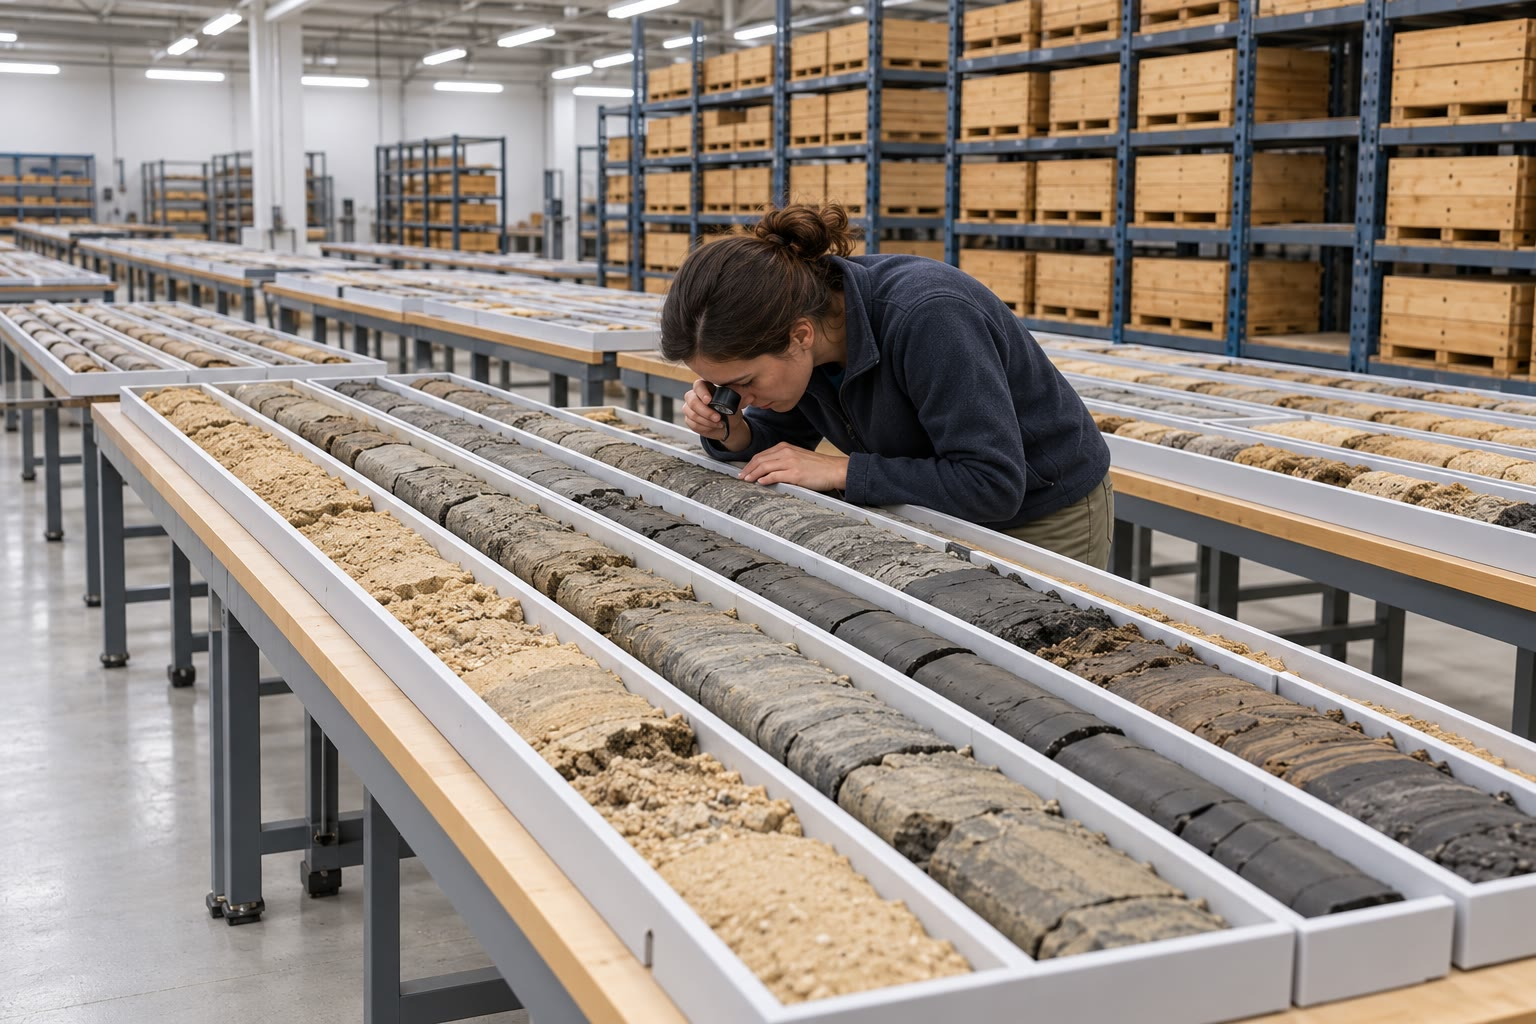
\includegraphics[width=\linewidth]{images/book5/ai/b3-core-store.jpg}

{\scriptsize कोर-भंडार: रेत और पंक के विभाजित क्रोड ट्रे में, एक भूवैज्ञानिक
हाथ-लेंस लिए हुए। AI से बनाया गया चित्रण।}
\end{minipage}
\end{inthelab}

\section{अभ्यास}

\begin{exercise}[$\star$]\label{exo:b3:facies-models:1}
एक क्रोड आधार से ऊपर की ओर यह दिखाता है: अपतटीय पंक, परस्पर-स्तरित पंक और महीन रेत,
\omterm{def:b3:facies-models:shoreface}{तटमुख} रेत, पुलिन रेत, फिर जड़ों वाला कोयला। वॉल्थर के नियम का उपयोग करके
उस समय तट के साथ परिवेशों का क्रम दीजिए, और वह दिशा बताइए जिसमें
तटरेखा खिसकी। ट्रांसग्रेशन से क्या छूटा होगा?
\end{exercise}

\begin{exercise}[$\star$]\label{exo:b3:facies-models:2}
तीन रेत-निकायों के गामा-किरण आकार दिए गए हैं: (क) \qty{8}{m} मोटी एक घंटी
जिसका आधार तीखा है; (ख) \qty{20}{m} मोटी एक कीप; (ग) \qty{30}{m} मोटा एक बेलन
जिसका शीर्ष और आधार तीखे हैं। प्रत्येक के लिए एक परिवेश सुझाइए, और
कोर में वह अवलोकन बताइए जो उसकी पुष्टि करेगा।
\end{exercise}

\begin{exercise}[$\star$]\label{exo:b3:facies-models:3}
एक बलुआ पत्थर का $\rho_b = \qty{2.40}{g/cm^3}$ है। क्वार्ट्ज़ आव्यूह और मीठे पानी के साथ इसकी छिद्रता परिकलित कीजिए, फिर
\qty{1.1}{g/cm^3} के लवण-जल के साथ।
\end{exercise}
% ledger: keys:density-porosity

\begin{exercise}[$\star$]\label{exo:b3:facies-models:4}
\qty{75}{m} और \qty{110}{m} के प्रमुख तरंगदैर्घ्य वाली तरंगें (बोय अध्ययन के
संरक्षित और खुले समुद्र)। अनुमान लगाइए कि प्रत्येक किस गहराई पर
अपनी सतही गति का \qty{4}{\percent} बनाए रखती है, और
\qty{20}{m} की गहराई पर शेष भाग का अंश परिकलित कीजिए।
\end{exercise}
% ledger: losspeters10:wavebase

\begin{exercise}[$\star\star$]\label{exo:b3:facies-models:5}
एक चूना-पत्थर का $\Delta t = \qty{60}{\micro\second/ft}$ है। समय-औसत समीकरण से
47.6 और \qty{52.6}{\micro\second/ft} के आव्यूह के लिए तथा
\qty{189}{\micro\second/ft} पर लवण-जल के लिए इसकी छिद्रता परिकलित कीजिए।
इस अंतर से क्या सीख मिलती है?
\end{exercise}
% ledger: keys:sonic

\begin{exercise}[$\star\star$]\label{exo:b3:facies-models:6}
एक \qty{40}{m} के अंतराल में कटऑफ़ से नीचे 6.0, 3.5, 8.0 और \qty{2.5}{m} मोटे
रेत-संस्तर हैं, शेष पंक है। इसका \omterm{def:b3:facies-models:ntg}{शुद्ध-से-सकल अनुपात} परिकलित कीजिए।
रेत में \qty{22}{\percent} छिद्रता हो, तो अंतराल के एक
वर्ग किलोमीटर में कितना रंध्र आयतन होता है?
\end{exercise}

\begin{exercise}[$\star\star$]\label{exo:b3:facies-models:7}
कैन्यन के मुहाने के पास एक गंदलाव-निक्षेप संस्तर \qty{1.2}{m} संहत रेत (Ta) है,
जिसका ऊपरी भाग अगले संस्तर द्वारा अपरदित है; \qty{30}{km} दूर जलमग्न पंखे में उसी प्रवाह का
एक संस्तर \qty{3}{cm} पंक की परत के नीचे \qty{8}{cm} लहरिका-स्तरित महीन रेत और गाद है।
प्रत्येक के विभाजन बताइए और परिवर्तन की व्याख्या कीजिए।
\end{exercise}

\begin{exercise}[$\star\star$]\label{exo:b3:facies-models:8}
\qty{9}{m} मोटा एक \omterm{def:b3:facies-models:association}{ऊपर की ओर महीन होता अनुक्रम} है, जिसके तीखे आधार पर कंकड़,
तिर्यक संस्तरित रेत, लहरिकायुक्त महीन रेत और मूल वाला पंक है। इसकी व्याख्या कीजिए,
और उस वाहिका की गहराई का अनुमान लगाइए जिसने इसे बनाया। क्या वॉल्थर का नियम इसके
आधार के आर-पार लागू हो सकता है? क्यों?
\end{exercise}

\begin{exercise}[$\star\star$]\label{exo:b3:facies-models:9}
एक प्लेटफ़ॉर्म का तल \qty{40}{km} में \qty{60}{m} गिरता है; दूसरा
\qty{30}{km} तक \qty{5}{m} की गहराई बनाए रखता है, फिर \qty{1.5}{km} में \qty{300}{m} गिरता है।
दोनों प्रवणताएँ परिकलित कीजिए, प्रत्येक प्लेटफ़ॉर्म का नाम बताइए, और दूसरे के
किनारे पर अपेक्षित संलक्षणी बताइए।
\end{exercise}

\begin{exercise}[$\star\star\star$]\label{exo:b3:facies-models:10}
एक तटरेखा $v$ की गति से आगे बढ़ती है, जबकि सापेक्ष समुद्र-तल
$A$ की दर से उठता है, और उसकी \omterm{def:b3:facies-models:shoreface}{तटमुख} पट्टी $w$ चौड़ी है। दिखाइए कि
ऊर्ध्वाधर अनुक्रम में \omterm{def:b3:facies-models:shoreface}{तटमुख} रेत की मोटाई $h = wA/v$ है। इसे $w = \qty{2}{km}$,
$A = \qty{0.2}{m/kyr}$ और $v = \qty{20}{m/kyr}$ के लिए परिकलित कीजिए, और बताइए कि
$A = 0$ होने पर क्या होता है। अध्याय~\ref{ch:b3:sequence-stratigraphy} के
\omterm{def:b3:sequence-stratigraphy:trajectory}{तटरेखा प्रक्षेप-पथ} पर प्रतिज्ञप्ति से तुलना कीजिए।
\end{exercise}

\begin{exercise}[$\star\star\star$]\label{exo:b3:facies-models:11}
एक बलुआ पत्थर का $\rho_b = \qty{2.30}{g/cm^3}$ और $\Delta t =
\qty{86}{\micro\second/ft}$ है। क्वार्ट्ज़ बलुआ-पत्थर आव्यूह के साथ प्रत्येक लॉग से
(2.65, \qty{52.6}{\micro\second/ft}) और लवण-जल (घनत्व के लिए 1.0,
\qty{189}{\micro\second/ft}) लेकर इसकी छिद्रता परिकलित कीजिए। यदि ध्वनिक छिद्रता सही है, तो
\omterm{def:b3:facies-models:wireline}{घनत्व-लॉग} से कौन-सा कण-घनत्व निहित होता है, और सीमेंट क्या हो सकता है?
\end{exercise}
% ledger: keys:density-porosity, keys:sonic

\begin{exercise}[$\star\star\star$]\label{exo:b3:facies-models:12}
एक कोर में काला अपतटीय पंक सीधे मूल वाले कोयले पर टिका है, और संपर्क पर
सीपों के मलबे की एक पतली परत है। समझाइए कि इसके आर-पार वॉल्थर का नियम क्यों
लागू नहीं होता, वह कौन-सी सतह है, और तटीय अनुक्रम का कितना भाग
लुप्त हो सकता है, यदि तटरेखा के गुज़रते समय तरंगों ने तल को \omterm{def:b3:facies-models:shoreface}{सामान्य-मौसम
तरंग-आधार} लगभग \qty{10}{m} तक अपरदित कर दिया हो।
\end{exercise}

\section{समस्या: वार्डन-2, आवरण के आर-पार एक कुआँ}

\begin{problem}[{सप्ताहांत समस्या --- एक काल्पनिक कुएँ के लॉग, छिद्रता, संलक्षणी और शुद्ध रेत,
वार्डन अभिनति में}]
\label{pb:b3:facies-models:1}
कुआँ वार्डन-2 वार्डन पहाड़ियों की अभिनति में, क्षेत्र के ग्रिड पर (7500, 7000) पर
खोदा गया है, जिसकी भू-उन्नति
\qty{441.0}{m} है, और कुल गहराई \qty{1200}{m} तक है। इसके लॉग अंतिम खंड के चित्र में अंकित हैं।
कण-घनत्व 2.65 (क्वार्ट्ज़) और
\qty{2.71}{g/cm^3} (कैल्साइट), रंध्र-जल का \qty{1.0}{g/cm^3}, आव्यूह के
पारगमन काल 52.6 (बलुआ पत्थर) और \qty{47.6}{\micro\second/ft}
(चूना-पत्थर), तथा जल के लिए \qty{189}{\micro\second/ft} लीजिए।

\medskip\noindent\textbf{भाग I --- लॉग पढ़ना।}
\begin{enumerate}
\item गामा-किरण 12 से \qty{110}{API} तक \qty{766}{m} पर उछलती है,
  \qty{866}{m} पर 18 तक गिरती है, \qty{1046}{m} से अनियमित हो जाती है और
  \qty{1166}{m} से \qty{85}{API} पर स्थिर रहती है। मिली इकाइयों के नाम उनके लॉग से बताइए।
\item आवरण की प्रत्येक इकाई की मोटाई और
  आवरण के आधार की उन्नति परिकलित कीजिए।
\item सतह के पास चॉक का घनत्व \qty{2.03}{g/cm^3} है, और
  \qty{750}{m} पर यह \qty{2.36}{g/cm^3} है। दोनों गहराइयों पर इसकी छिद्रता परिकलित कीजिए।
  गहराई के साथ चॉक का क्या होता है?
\item शेल को उसके घनत्व से छिद्रता क्यों नहीं दी जाती?
\item शिस्ट \qty{2.75}{g/cm^3} और \qty{50}{\micro\second/ft} पढ़ता है।
  तेज़, सघन और अछिद्र आधारशैल ड्रिलर को क्या बताती है?
\end{enumerate}

\medskip\noindent\textbf{भाग II --- छिद्रता।}
\begin{enumerate}[resume]
\item चूना-पत्थर \qty{2.573}{g/cm^3} पढ़ता है: इसकी घनत्व-छिद्रता परिकलित कीजिए।
\item यह \qty{58.9}{\micro\second/ft} पढ़ता है: इसकी ध्वनिक छिद्रता परिकलित कीजिए और
  तुलना कीजिए।
\item वाहिका के भरावों की स्वच्छ रेत \qty{2.32}{g/cm^3} पढ़ती है: इसकी
  छिद्रता परिकलित कीजिए।
\item इसे इसके पारगमन काल \qty{79.9}{\micro\second/ft} से जाँचिए।
\item यदि रंध्र-जल \qty{1.1}{g/cm^3} का लवण-जल होता, तो रेत की घनत्व-छिद्रता
  कितनी बदल जाती?
\item कौन-सी इकाई बेहतर जलभृत या भंडार बनाती, और
  उसके ऊपर वाली आवरण चट्टान कौन-सी होती?
\end{enumerate}

\medskip\noindent\textbf{भाग III --- संलक्षणी।} एक क्रोड, 1108 से
\qty{1124}{m} तक काटा गया, तल से दिखाता है: कीचड़-खंडों और कंकड़ों वाली एक अपरदित सतह;
\qty{10.4}{m} तिर्यक संस्तरित मध्यम रेत; \qty{3.2}{m} लहरिकायुक्त
महीन रेत जो गाद में बदलती है; \qty{2.4}{m} मूल-चिह्नों वाला लाल-भूरा कीचड़।
\begin{enumerate}[resume]
\item क्रोडित अंतराल में अपेक्षित गामा-किरण आकृति खींचिए।
\item प्रत्येक भाग का अनुक्रम और निक्षेपण-परिवेश नाम दीजिए।
\item वॉल्थर के नियम से उन परिवेशों का वर्णन कीजिए जो साथ-साथ पड़ते हैं।
\item वाहिका की गहराई का अनुमान लगाइए।
\item बलुआ पत्थर में ऐसी ग्यारह इकाइयाँ हैं, और प्रत्येक एक तीखे आधार पर है।
  इनका स्टैकिंग नदी और उसके मैदान के बारे में क्या बताता है?
\item क्या वॉल्थर के नियम से एक इकाई से अगली इकाई तक जाया जा सकता है? क्यों?
\end{enumerate}

\medskip\noindent\textbf{भाग IV --- शुद्ध रेत।} ग्यारह वाहिका-भराव,
बलुआ पत्थर के आधार से इनकी मोटाई क्रमशः 14, 9, 12, 7, 16, 10, 13, 8, 11, 12 और
\qty{8}{m} मोटी है। प्रत्येक इकाई स्वच्छ रेत (\qty{30}{API}) से शुरू होती है, जो
अपनी मोटाई के 0.60, 0.45, 0.55, 0.30, 0.65, 0.40, 0.55, 0.35, 0.50,
0.45 और 0.30 भाग में फैली है, फिर ऊपर की ओर महीन होती है, इसका भाग 0.25, 0.30, 0.25, 0.40,
0.20, 0.30, 0.25, 0.35, 0.25, 0.30 और 0.35 है, गामा-किरण रैखिक रूप से
\qty{105}{API} तक बढ़ती है, और कीचड़ में समाप्त होती है।
\begin{enumerate}[resume]
\item प्रत्येक महीन होते अंतराल का कौन-सा भाग \qty{60}{API}
  सीमा-मान से नीचे पड़ता है?
\item सबसे निचली इकाई और सबसे मोटी इकाई की शुद्ध रेत परिकलित कीजिए।
\item बलुआ पत्थर का स्वच्छ-रेत कुल और
  महीन होते अंतराल का कुल परिकलित कीजिए।
\item इसका \omterm{def:b3:facies-models:ntg}{शुद्ध-से-सकल अनुपात} परिकलित कीजिए।
\item सीमा-मान 45 या
  \qty{75}{API} होने पर शुद्ध रेत कैसे बदलेगी?
\item प्रश्न 8 की रेत की छिद्रता के साथ, शुद्ध रेत का रंध्र-आयतन
  एक वर्ग किलोमीटर के नीचे परिकलित कीजिए।
\item वार्डन-2 पर ट्राइऐसिक बलुआ पत्थर की शुद्ध रेत मोटाई बताइए।
\end{enumerate}
\end{problem}
% ledger: keys:density-porosity, keys:sonic, keys:gamma
